\documentclass[a4paper, 12pt]{article}
\usepackage[left=2cm,right=2cm,
    top=3cm,bottom=3cm,bindingoffset=0cm]{geometry}
%%% Работа с русским языком
\usepackage{cmap}					% поиск в PDF
\usepackage{mathtext} 				% русские буквы в формулах
\usepackage[T2A]{fontenc}			% кодировка
\usepackage[utf8]{inputenc}			% кодировка исходного текста
\usepackage[english,russian]{babel}	% локализация и переносы
\usepackage{xcolor}
\usepackage{hyperref}
 % Цвета для гиперссылок
\definecolor{linkcolor}{HTML}{799B03} % цвет ссылок
\definecolor{urlcolor}{HTML}{799B03} % цвет гиперссылок

\hypersetup{pdfstartview=FitH,  linkcolor=linkcolor,urlcolor=urlcolor, colorlinks=true}

%%% Дополнительная работа с математикой
\usepackage{amsfonts,amssymb,amsthm,mathtools} % AMS
\usepackage{amsmath}
\usepackage{icomma} % "Умная" запятая: $0,2$ --- число, $0, 2$ --- перечисление

%% Номера формул
%\mathtoolsset{showonlyrefs=true} % Показывать номера только у тех формул, на которые есть \eqref{} в тексте.

%% Шрифты
\usepackage{euscript}	 % Шрифт Евклид
\usepackage{mathrsfs} % Красивый матшрифт

%% Свои команды
\DeclareMathOperator{\sgn}{\mathop{sgn}}

%% Перенос знаков в формулах (по Львовскому)
\newcommand*{\hm}[1]{#1\nobreak\discretionary{}
{\hbox{$\mathsurround=0pt #1$}}{}}
% графика
\usepackage{graphicx}
\graphicspath{{pictures/}}
\DeclareGraphicsExtensions{.pdf,.png,.jpg}
\author{Бурмашев Григорий, БПМИ-208}
\title{Дифференциальные уравнения, дз -- 2}
\date{\today}
\begin{document}
\maketitle
\clearpage
\section*{Номер 1}
Если дано комплексное число $z$:
\[
z = x + iy
\]

\begin{itemize}
\item Тригонометрическая форма:
\[
z = |z| (\cos \varphi + i \sin \varphi)
\]
Где:
\[
|z| = \sqrt{x^2 + y^2}
\]
\[
\cos \varphi = \frac{x}{|z|}
\]
\[
\sin \varphi = \frac{y}{|z|}
\]
А если $x > 0, y > 0$, то можно как:
\[
\varphi = \arctg \frac{y}{x}
\]
\item Показательная форма:
\[
z = |z| \cdot e^{i \varphi}
\]
\end{itemize}
\clearpage
\subsection*{1)}
\[
z = 1 + \sqrt{3} i
\]
Находим тригонометрическую форму:
\[
|z| = \sqrt{1 + 3 } =  \sqrt{4} = 2
\]
\[
\cos \varphi = \frac{1}{2}
\]
\[
\sin \varphi = \frac{\sqrt{3}}{2}
\]
Отсюда
\[
\varphi = \frac{\pi}{3}
\]
Итого:
\[
z = 2 \left(
\cos \frac{\pi}{3}
+ 
i
\sin \frac{\pi}{3}
\right)
\]
Находим показательную форму:
\[
z = 2 e^{i \frac{\pi}{3}}
\]
\begin{center}
\textbf{Ответ: } 
\[
2 \left(
\cos \frac{\pi}{3}
+ 
i
\sin \frac{\pi}{3}
\right)
\]
\[
2 e^{i \frac{\pi}{3}}
\]
\end{center}
\clearpage
\subsection*{2)}
\[
z = 2i
\]
Находим тригонометрическую форму:
\[
|z| = \sqrt{0 + 4} = 2
\]
\[
\cos \varphi = 0
\]
\[
\sin \varphi = \frac{2}{2} = 1
\]
Отсюда
\[
\varphi = \frac{\pi}{2}
\]
Итого:
\[
z = 2  \left(
\cos  \frac{\pi}{2}
+ 
i
\sin  \frac{\pi}{2}
\right)
\]
Находим показательную форму:
\[
z = 2 e^{i \frac{\pi}{2}}
\]
\begin{center}
\textbf{Ответ: } 
\[
2  \left(
\cos  \frac{\pi}{2}
+ 
i
\sin  \frac{\pi}{2}
\right)
\]
\[
2 e^{i \frac{\pi}{2}}
\]
\end{center}
\clearpage
\subsection*{3)}
\[
z = -7i
\]
Находим тригонометрическую форму:
\[
|z| = \sqrt{49} = 7
\]
\[
\cos \varphi = 0
\]
\[
\sin \varphi = - \frac{7}{7} = -1
\]
Отсюда
\[
\varphi = -\frac{\pi}{2}
\]
Итого:
\[
z = 7  \left(
\cos  \left( -\frac{\pi}{2} \right)
+ 
i
\sin  \left( -\frac{\pi}{2} \right)
\right)
\]
Находим показательную форму:
\[
z = 7 e^{-i\frac{\pi}{2}}
\]
\begin{center}
\textbf{Ответ: } 
\[
7  \left(
\cos  \left( -\frac{\pi}{2} \right)
+ 
i
\sin  \left( -\frac{\pi}{2} \right)
\right)
\]
\[
7 e^{-i\frac{\pi}{2}}
\]
\end{center}
\clearpage
\subsection*{4)}
\[
z = 1 - \sqrt{3}i 
\]
Находим тригонометрическую форму:
\[
|z| = \sqrt{1 + 3} = 2
\]
\[
\cos \varphi = \frac{1}{2}
\]
\[
\sin \varphi = -\frac{\sqrt{3}}{2}
\]
Отсюда
\[
\varphi = -\frac{\pi}{3}
\]
Итого:
\[
z = 2  \left(
\cos  \left( -\frac{\pi}{3} \right)
+ 
i
\sin  \left( -\frac{\pi}{3} \right)
\right)
\]
Находим показательную форму:
\[
z = 2 e^{-i \frac{\pi}{3}}
\]
\begin{center}
\textbf{Ответ: } 
\[
2  \left(
\cos  \left( -\frac{\pi}{3} \right)
+ 
i
\sin  \left( -\frac{\pi}{3} \right)
\right)
\]
\[
 2 e^{-i \frac{\pi}{3}}
\]
\end{center}
\clearpage
\subsection*{5)}
\[
z = \sqrt{3} i
\]
Находим тригонометрическую форму:
\[
|z| = \sqrt{3}
\]
\[
\cos \varphi = 0
\]
\[
\sin \varphi = 1
\]
Отсюда
\[
\varphi = \frac{\pi}{2}
\]
Итого:
\[
z = \sqrt{3}  \left(
\cos  \left( \frac{\pi}{2} \right)
+ 
i
\sin  \left( \frac{\pi}{2} \right)
\right)
\]
Находим показательную форму:
\[
z = \sqrt{3} e^{i \frac{\pi}{2}}
\]
\begin{center}
\textbf{Ответ: } 
\[
\sqrt{3}  \left(
\cos  \left( \frac{\pi}{2} \right)
+ 
i
\sin  \left( \frac{\pi}{2} \right)
\right)
\]
\[
 \sqrt{3} e^{i \frac{\pi}{2}}
\]
\end{center}
\clearpage
\subsection*{6)}
\[
z = 3 + 4i
\]
Находим тригонометрическую форму:
\[
|z| = \sqrt{9 + 16} = 5
\]
Т.к $3 > 0, 4 > 0$, то:
\[
\varphi = \arctg \frac{4}{3}
\]
Итого:
\[
z = 5 \left(
\cos 
\left(
\arctg  \left( \frac{4}{3} \right)
\right)
+ 
i
\sin 
\left(
\arctg  \left( \frac{4}{3} \right)
\right)
\right)
\]
Находим показательную форму:
\[
z = 5 e^{i \arctg \left( \frac{4}{3} \right)}
\]
\begin{center}
\textbf{Ответ: } 
\[
5 \left(
\cos 
\left(
\arctg  \left( \frac{4}{3} \right)
\right)
+ 
i
\sin 
\left(
\arctg  \left( \frac{4}{3} \right)
\right)
\right)
\]
\[
5 e^{i \arctg \left( \frac{4}{3} \right)}
\]
\end{center}
\clearpage
\section*{Номер 2}
Если есть комплексное число $z$ и есть его тригонометрическая форма, то у нас есть формула: 
\[
\sqrt[n]{z}
=
\sqrt[n]{|z|}
\cdot
\left(
\cos 
\left(
\frac{\varphi + 2 \pi k}{n}
\right)
+
i
\sin
\left(
\frac{\varphi + 2 \pi k}{n}
\right)
\right)
\]
А корней всегда будет $n$ штук, т.е в данном случае $k \in \{0, 1, 2, \ldots, n - 1\}$
\subsection*{1)}
\[
(1 + \sqrt{3}i)^{\frac{1}{2}}
\]
\[
z = 1 + \sqrt{3}i
\]
Тригонометрическую форму уже посчитали:
\[
z
=
2 \left(
\cos \frac{\pi}{3}
+ 
i
\sin \frac{\pi}{3}
\right)
\]
В данном случае $n = 2$, поэтому $k \in \{0, 1\}$. Теперь извлекаем по формуле:
\[
\sqrt[2]{z} = \sqrt{2}
 \left(
\cos 
\left(
\frac{ \frac{\pi}{3}+ 2 \pi k}{2}
\right)
+
i
\sin
\left(
\frac{ \frac{\pi}{3}+ 2 \pi k}{2}
\right)
\right)
\]
\[
\sqrt[2]{z} = \sqrt{2}
 \left(
\cos 
\left(
\frac{\pi}{6} + \pi k
\right)
+
i
\sin
\left(
\frac{\pi}{6} + \pi k
\right)
\right)
\]
\begin{center}
\textbf{Ответ: } 

Общий вид:
\[
 \sqrt{2}
 \left(
\cos 
\left(
\frac{\pi}{6} + \pi k
\right)
+
i
\sin
\left(
\frac{\pi}{6} + \pi k
\right)
\right)
\]
Множество:
\[
k \in \{0, 1\}
\]
\end{center}

\clearpage
\subsection*{2)}
\[
(2i)^{\frac{1}{3}}
\]
\[
z = 2i
\]
Тригонометрическую форму уже посчитали:
\[
z
=
2  \left(
\cos  \frac{\pi}{2}
+ 
i
\sin  \frac{\pi}{2}
\right)
\]
В данном случае $n = 3$, поэтому $k = \in \{0, 1, 2\}$. Теперь извлекаем по формуле:
\[
\sqrt[3]{z} = \sqrt[3]{2}
 \left(
\cos 
\left(
\frac{ \frac{\pi}{2}+ 2 \pi k}{3}
\right)
+
i
\sin
\left(
\frac{ \frac{\pi}{2}+ 2 \pi k}{3}
\right)
\right)
\]
\[
\sqrt[3]{z} = \sqrt[3]{2}
 \left(
\cos 
\left(
\frac{\pi}{6} + \frac{2\pi}{3} k
\right)
+
i
\sin
\left(
\frac{\pi}{6} + \frac{2\pi}{3} k
\right)
\right)
\]
\begin{center}
\textbf{Ответ: } 

Общий вид:
\[
\sqrt[3]{z} = \sqrt[3]{2}
 \left(
\cos 
\left(
\frac{\pi}{6} + \frac{2\pi}{3} k
\right)
+
i
\sin
\left(
\frac{\pi}{6} + \frac{2\pi}{3} k
\right)
\right)
\]
Множество:
\[
k \in \{0, 1, 2\}
\]
\end{center}
\clearpage
\subsection*{3)}
\[
(-7i)^{\frac{1}{6}}
\]
\[
z = -7i
\]
Тригонометрическую форму уже посчитали:
\[
z
=
7  \left(
\cos  \left( -\frac{\pi}{2} \right)
+ 
i
\sin  \left( -\frac{\pi}{2} \right)
\right)
\]
В данном случае $n = 6$, поэтому $k \in \{0, 1, \ldots, 5\}$. Теперь извлекаем по формуле:
\[
\sqrt[6]{z} = \sqrt[6]{7}
 \left(
\cos 
\left(
\frac{ -\frac{\pi}{2}+ 2 \pi k}{6}
\right)
+
i
\sin
\left(
\frac{ -\frac{\pi}{2}+ 2 \pi k}{6}
\right)
\right)
\]
\[
\sqrt[6]{z} = \sqrt[6]{7}
 \left(
\cos 
\left(
-\frac{\pi}{12} + \frac{\pi}{3} k
\right)
+
i
\sin
\left(
-\frac{\pi}{12} + \frac{\pi}{3} k
\right)
\right)
\]
\begin{center}
\textbf{Ответ: } 

Общий вид:
\[
\sqrt[6]{z} = \sqrt[6]{7}
 \left(
\cos 
\left(
-\frac{\pi}{12} + \frac{\pi}{3} k
\right)
+
i
\sin
\left(
-\frac{\pi}{12} + \frac{\pi}{3} k
\right)
\right)
\]
Множество:
\[
k \in \{0, 1, \ldots, 5\}
\]
\end{center}
\clearpage
\subsection*{4)}
Найти частное от деления:
\[
\frac{23 + i}{3 + i}
\]
Для этого домножим числитель и знаменатель на сопряженное знаменателю, т.е на $3 - i$:
\[
\frac{23 + i}{3 + i}
=
\frac{23 + i}{3 + i} 
\cdot
\frac{3 - i}{3- i} 
=
\frac{(23 +i) (3 - i)}{3^2 + 1^2}
=
\frac{70 - 20i}{10}
= 7 - 2i
\]
\begin{center}
\textbf{Ответ: } 
\[
7 - 2i
\]
\end{center}
\clearpage
\section*{Номер 3}
\subsection*{a)}
\[
y^{(5)}  - 6y^{(4)} + 9y^{'''} = 0
\]
Смотрим на характеристический многочлен:
\[
P(\lambda) = \lambda^5 - 6 \lambda^4 + 9 \lambda^3
\]
Рассмотрим уравнение $P(\lambda) = 0$:
\[
\lambda^5 - 6 \lambda^4 + 9 \lambda^3 = 0
\]
\[
\lambda^3(\lambda^2 - 6\lambda + 9) = 0
\]
\[
\lambda^3 (\lambda - 3)^2 = 0
\]
Отсюда корни:
\[
\lambda_1 = 0, \lambda_2 = 3
\]
У $\lambda_1$ кратность 3, отсюда получаем решения:
\[
      \begin{gathered} 
e^{0x}  = 1 \\
x e^{0x} = x \\
x^2 e^{0x} = x^2
      \end{gathered} 
\]
У $\lambda_2$ кратность 2, отсюда получаем решения:
\[
      \begin{gathered} 
e^{3x} \\
xe^{3x} \\
      \end{gathered} 
\]
Итого решение:
\[
C_1 + C_2 x + C_3 x^2 + C_4 e^{3x} + C_5 xe^{3x}
\]
\begin{center}
\textbf{Ответ: } 
\[
y = C_1 + C_2 x + C_3 x^2 + C_4 e^{3x} + C_5 xe^{3x}
\]
\end{center}
\clearpage
\subsection*{b)}
\[
y^{'''} - y^{''} - y' + y = 0
\]
Смотрим на характеристический многочлен:
\[
P(\lambda) = \lambda^3 - \lambda^2 -  \lambda + 1
\]
Рассмотрим уравнение $P(\lambda) = 0$:
\[
\lambda^3 - \lambda^2 -  \lambda + 1 = 0
\]
Угадывается корень 1, далее делением на $\lambda - 1$ получаем:
\[
 (\lambda - 1) (\lambda - 1)(\lambda + 1)= 0
\]
\[
(\lambda -1)^2 (\lambda + 1) = 0
\]
Отсюда корни:
\[
\lambda_1 = 1, \lambda_2 = -1
\]
У $\lambda_1$ кратность 2, отсюда получаем решения:
\[
      \begin{gathered} 
e^{x}  \\
x e^{x} 
      \end{gathered} 
\]
У $\lambda_2$ кратность 1, отсюда получаем решение:
\[
      \begin{gathered} 
e^{-x} \\
      \end{gathered} 
\]
Итого решение:
\[
C_1e^x + C_2 xe^x + C_3e^{-x}
\]
\begin{center}
\textbf{Ответ: } 
\[
y = C_1e^x + C_2 xe^x + C_3e^{-x}
\]
\end{center}
\clearpage
\subsection*{c)}
\[
y^{(4)} + 4y'' +3y = 0
\]
Смотрим на характеристический многочлен:
\[
P(\lambda) = \lambda^4 + 4\lambda^2 + 3
\]
Рассмотрим уравнение $P(\lambda) = 0$:
\[
\lambda^4 + 4\lambda^2 + 3 = 0
\]
\[
(\lambda^2 + 1)(\lambda^2 + 3) = 0
\]
Придется работать с комплексными корнями, так что считаем для первой скобки:
\[
\lambda^2 = - 1 + 0i,  \;
|\lambda^2| = \sqrt{1} = 1,  \;
 \varphi = \pi 
\]
\[
\sqrt{\lambda^2} = 
\left(
\cos 
\left(
\frac{\pi + 2 \pi k}{2}
\right)
+i
\sin
\left(
\frac{\pi + 2 \pi k}{2}
\right)
\right), k \in \{0, 1\}
\]
\[
k = 0 : \cos \left(\frac{\pi}{2}\right) + i\sin \left(\frac{\pi}{2}\right)  = 0 + i = i
\]
\[
k = 1 : \cos \left(\frac{\pi}{2} + \pi \right) + i\sin \left(\frac{\pi}{2}+\pi \right) = 0 - i = -i
\]
Отсюда получили первые два корня:
\[
\lambda_1 = i, \lambda_2 = -i
\]
Теперь считаем тоже самое, но для второй скобки:
\[
\lambda^2 = -3 + 0i,  \;
|\lambda^2| = \sqrt{3}, \;
\varphi = \pi 
\]
\[
\sqrt{\lambda^2} = 
\sqrt{3}
\left(
\cos 
\left(
\frac{\pi + 2 \pi k}{2}
\right)
+i
\sin
\left(
\frac{\pi + 2 \pi k}{2}
\right)
\right), k \in \{0, 1\}
\]
\[
k = 0 :\sqrt{3} \cos \left(\frac{\pi}{2}\right) + i\sin \left(\frac{\pi}{2}\right)  = \sqrt{3}(0 + i) =\sqrt{3} i
\]
\[
k = 1 :\sqrt{3} \cos \left(\frac{\pi}{2} + \pi \right) + i\sin \left(\frac{\pi}{2}+\pi \right) = \sqrt{3}(0 - i) = \sqrt{3}(-i)
\]
И еще два корня:
\[
\lambda_3 = \sqrt{3}i, \lambda_4 = -\sqrt{3}i
\]
Теперь обьединяем решения:
\[
\lambda_1 = \pm i, \lambda_2 = \pm \sqrt{3} i
\]
С семинара:
\begin{center}
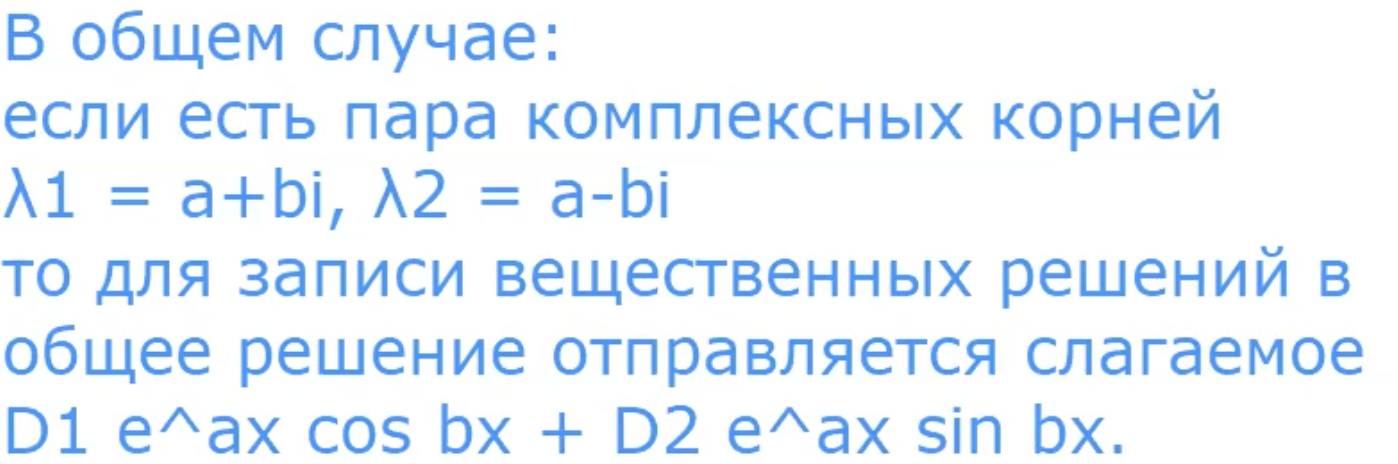
\includegraphics[scale=0.2]{1.png}
\end{center}
Тогда получаем решение:
\[
y = D_1 e^{0x} \cos(x) + D_2 e^{0x} \sin(x) +  D_3 e^{0x} \cos(\sqrt{3}x) +  D_4 e^{0x} \sin(\sqrt{3}x)
\]
Итого:
\[
y = D_1 \cos(x) + D_2\sin(x) +  D_3 \cos(\sqrt{3}x) +  D_4  \sin(\sqrt{3}x)
\]
\begin{center}
\textbf{Ответ: } 
\[
y = D_1 \cos(x) + D_2\sin(x) +  D_3 \cos(\sqrt{3}x) +  D_4  \sin(\sqrt{3}x)
\]
\end{center}
\clearpage
\subsection*{d)}
\[
y^{'''} - 3y^{'} +2y = 0
\]
Смотрим на характеристический многочлен:
\[
P(\lambda) = \lambda^3 - 3\lambda + 2
\]
Рассмотрим уравнение $P(\lambda) = 0$:
\[
\lambda^3 - 3\lambda + 2 = 0
\]
Угадывается корень 1, далее делением на $\lambda - 1$ получаем:
\[
 (\lambda -1) (\lambda + 2)(\lambda - 1)= 0
\]
\[
(\lambda -1)^2 (\lambda + 2) = 0
\]
Отсюда корни:
\[
\lambda_1 = 1, \lambda_2 = -1
\]
У $\lambda_1$ кратность 2, отсюда получаем решения:
\[
      \begin{gathered} 
e^{x}  \\
x e^{x} 
      \end{gathered} 
\]
У $\lambda_2$ кратность 1, отсюда получаем решение:
\[
      \begin{gathered} 
e^{-2x} \\
      \end{gathered} 
\]
Итого решение:
\[
C_1e^x + C_2 xe^x + C_3e^{-2x}
\]
\begin{center}
\textbf{Ответ: } 
\[
y = C_1e^x + C_2 xe^x + C_3e^{-2x}
\]
\end{center}
\clearpage
\subsection*{e)}
\[
y^{(6)} + 64y = 0
\]
Смотрим на характеристический многочлен:
\[
P(\lambda) = \lambda^6  + 64 = 0
\]
Рассмотрим уравнение $P(\lambda) = 0$:
\[
\lambda^6 + 64= 0
\]
Переходим в комплексные и ищем корни:
\[
\lambda^6 = -64 +0i, |\lambda^6| = \sqrt{64^2} = 64, \varphi = \pi
\]
\[
\sqrt[6]{\lambda^6} =
\sqrt[6]{64}
\left(
\cos 
\left(
\frac{\pi + 2 \pi k}{6}
\right)
+i
\sin
\left(
\frac{\pi + 2 \pi k}{6}
\right)
\right), k \in \{0, 1, \ldots, 5\}
\]
\[
\sqrt[6]{\lambda^6} =
2
\left(
\cos 
\left(
\frac{\pi}{6} + \frac{\pi}{3} k
\right)
+i
\sin
\left(
\frac{\pi}{6} + \frac{\pi}{3} k
\right)
\right), k \in \{0, 1, \ldots, 5\}
\]
Эх, перебираем все $k$:
\begin{flushleft}
\begin{equation*}
\begin{gathered}
k = 0:
 2 \left( \cos  \left(
\frac{\pi}{6}
\right) 
+ i \sin \left(
\frac{\pi}{6}
\right) \right)
=
2 \left(
\frac{\sqrt{3}}{2} + i\frac{1}{2}
\right)
=
\sqrt{3} + i 
\\
k = 1:
 2 \left( \cos  \left(
\frac{\pi}{6} + \frac{\pi}{3}
\right) 
+ i \sin \left(
\frac{\pi}{6} + \frac{\pi}{3}
\right) \right)
=
2 \left(
0 + i
\right)
=2i 
\\
k = 2:
 2 \left( \cos  \left(
\frac{\pi}{6} + \frac{\pi}{3} 2
\right) 
+ i \sin \left(
\frac{\pi}{6} + \frac{\pi}{3} 2
\right) \right)
=
2 \left(
-\frac{\sqrt{3}}{2} + i\frac{1}{2}
\right)
=
-\sqrt{3} + i
\\
k = 3:
 2 \left( \cos  \left(
\frac{\pi}{6} + \frac{\pi}{3} 3
\right) 
+ i \sin \left(
\frac{\pi}{6} + \frac{\pi}{3} 3
\right) \right)
=
2 \left(
-\frac{\sqrt{3}}{2} - i\frac{1}{2}
\right)
=
-\sqrt{3} -i
\\
 k = 4:
 2 \left( \cos  \left(
\frac{\pi}{6} + \frac{\pi}{3} 4
\right) 
+ i \sin \left(
\frac{\pi}{6} + \frac{\pi}{3} 4
\right) \right)
=
2 \left(
0 - i
\right)
= -2i
\\
k = 5:
 2 \left( \cos  \left(
\frac{\pi}{6} + \frac{\pi}{3} 5
\right) 
+ i \sin \left(
\frac{\pi}{6} + \frac{\pi}{3} 5
\right) \right)
=
2 \left(
\frac{\sqrt{3}}{2} - i \frac{1}{2}
\right)
=
\sqrt{3} - i
\end{gathered}
\end{equation*}
\end{flushleft}
Обьединяем попарно корни:
\[
\lambda_1 =  \sqrt{3} \pm i, \; \lambda_2 =  \pm 2i, \; \lambda_3 =  -\sqrt{3} \pm i
\]
Получаем итоговый ответ:
\[
y = D_1 e^{\sqrt{3} x} \cos x 
+
D_2 e^{\sqrt{3} x} \sin x
+
D_3 \cos 2x
+
D_4 \sin 2x
+
D_5 e^{-\sqrt{3} x} \cos x
+
D_6 e^{-\sqrt{3} x} \sin x
\]
\begin{center}
\textbf{Ответ: } 
\[
y = D_1 e^{\sqrt{3} x} \cos x 
+
D_2 e^{\sqrt{3} x} \sin x
+
D_3 \cos 2x
+
D_4 \sin 2x
+
D_5 e^{-\sqrt{3} x} \cos x
+
D_6 e^{-\sqrt{3} x} \sin x
\]
\end{center}
\clearpage
\section*{Номер 4}
\subsection*{a)}
\[
y'' + 4y = 2 \cos^2x
\]
Сначала решим однородное:
\[
y'' + 4y = 0
\]
Смотрим на характеристический многочлен:
\[
P(\lambda) = \lambda^2 + 4 
\]
Рассмотрим уравнение $P(\lambda) = 0$:
\[
\lambda^2 + 4 = 0
\]
\[
\lambda^2 = -4 + 0i, |\lambda^2| = \sqrt{16} = 4, \varphi = \pi
\]
\[
\sqrt{\lambda^2} = 
\sqrt{4} 
\left(
\cos 
\left(
\frac{\pi + 2 \pi k}{2}
\right)
+i
\sin
\left(
\frac{\pi + 2 \pi k}{2}
\right)
\right), k \in \{0, 1\}
\]
\[
k = 0 : 2(0 + i) = 2i 
\]
\[
k = 1: 2(0 - i) = -2i
\]
\[
\lambda = \pm 2i
\]
Получаем решение:
\[
\lambda_1 = \pm 2i
\]
И тогда:
\[
D_1 \cos (2x) + D_2 \sin (2x)
\]
Теперь ищем частное решение, вспоминаем формулу:
\[
2 \cos^2x = 1 + \cos 2x
\]
Начнем с $1$, это будет просто константа $d$:
\[
y_1 = d
\]
\[
y_1' = y_1'' = 0
\]
Тогда:
\[
0 + 4d = 1
\]
\[
d = \frac{1}{4}
\]
Теперь ищем второе. Корни у нас мнимые вида $\pm 2i$ с кратностью 1, у косинуса внутри $2$, значит  нужно домножить на $x$
\[
y_2 = x 
\left(
p \cdot \cos 2x + q \cdot \sin 2x
\right)
\]
\[
y_2' = p\cos 2x + q\cdot \sin 2x -2px \sin 2x  + 2 qx\cos 2x
\]
\[
y_2'' = 4q \cos 2x - 4px \cos 2x - 4 p \sin 2x  - 4 qx \sin 2x
\]
Тогда:
\[
4q \cos 2x - 4px \cos 2x - 4 p \sin 2x  - 4 qx \sin 2x + 4x(p \cos2x + q \sin 2x) = \cos 2x
\]
\[
4q \cos 2x -4 p \sin 2x = \cos 2x
\]
\[
\begin{cases}
4q = 1 \\
-4p = 0 
\end{cases}
\]
Отсюда
\[
\begin{cases}
q = \frac{1}{4} \\
p = 0
\end{cases}
\]
Т.е:
\[
y_2 = x(0 + \frac{1}{4} \sin 2x) = \frac{1}{4} \sin 2x
\]
Тогда общее решение:
\[
y = \frac{1}{4} + \frac{1}{4} \sin 2x + D_1 \cos (2x) + D_2 \sin (2x)
\]
\begin{center}
\textbf{Ответ: } 
\[
y = \frac{1}{4} + \frac{1}{4} \sin 2x + D_1 \cos (2x) + D_2 \sin (2x)
\]
\end{center}
\clearpage
\subsection*{b)}
\[
y''' - 3y' -2y = e^{-x}
\]
Сначала решим однородное:
\[
y''' - 3y' -2y= 0
\]
Смотрим на характеристический многочлен:
\[
P(\lambda) = \lambda^3 - 3 \lambda -2 
\]
Рассмотрим уравнение $P(\lambda) = 0$:
\[
\lambda^3 - 3 \lambda -2 = 0
\]
\[
(\lambda + 1)^2 (\lambda -2) = 0
\]
Получаем решения:
\[
\lambda_1 = -1, \lambda_2 = 2
\]
У $\lambda_1$ кратность 2, отсюда получаем решения:
\[
      \begin{gathered} 
e^{-x}  \\
x e^{-x}
      \end{gathered} 
\]
У $\lambda_2$ кратность 1, отсюда получаем решение:
\[
      \begin{gathered} 
e^{2x} \\
      \end{gathered} 
\]
Итого решение:
\[
C_1e^{-x} + C_2 xe^{-x} + C_3e^{2x}
\]
Теперь ищем частное решение, у $e^{-x}$ совпадение степени с $\lambda_1 = -1$, кратность равна 2, поэтому будет множитель $x^2$:
\[
y_1 = x^2 d e^{-x}
\]
\[
y_1' = 2x d e^{-x}  - d x^2 e^{-x} 
\]
\[
y_1'' = 2 d e^{-x} - 4 xd e^{-x}  + d x^2e^{-x} 
\]
\[
y_1''' = -x^2 d e^{-x} +6x d e^{-x} -6 d e^{-x}
\]
Подставляем:
\[
-x^2 d e^{-x} +6x d e^{-x} -6 d e^{-x} - 3(2x d e^{-x}  - d x^2 e^{-x} ) - 2x^2 de^{-x} = e^{-x}
\]
\[
-6de^{-x} = e^{-x}
\]
\[
d = -\frac{1}{6}
\]
Тогда:
\[
y_1 = - \frac{1}{6}x^2e^{-x}
\]
Отсюда получаем общее решение:
\[
 y = - \frac{1}{6}x^2e^{-x} + C_1e^{-x} + C_2 xe^{-x} + C_3e^{2x}
\]
\begin{center}
\textbf{Ответ: } 
\[
 y = - \frac{1}{6}x^2e^{-x} + C_1e^{-x} + C_2 xe^{-x} + C_3e^{2x}
\]
\end{center}
\clearpage
\subsection*{c)}
\[
y^{(4)} - y = e^x \cos x 
\]
Сначала решим однородное:
\[
y^{(4)} - y = 0
\]
Смотрим на характеристический многочлен:
\[
P(\lambda) = \lambda^4 - 1 
\]
Рассмотрим уравнение $P(\lambda) = 0$:
\[
 \lambda^4 - 1 = 0
\]
\[
(\lambda^2 - 1) (\lambda^2 + 1 ) = 0
\]
Получаем решения:
\[
\lambda_1 = 1, \lambda_2 = -1, \lambda_3 = \pm i 
\]
Итого решение:
\[
D_1 e^{x} + D_2 e^{-x} + D_3 \cos x + D_4 \sin x
\]
Теперь ищем частное решение, $a + bi =1 +  i$ -- не корень, значит будет $x^0$, поэтому:
\[
y_1 = e^x (r \cos x + t \sin x)
\]
\[
y_1 ' = e^x (r \cos x + t \sin x) + e^x (-r \sin x + t \cos x)
\]
\[
y_1'' =  e^x (r \cos x + t \sin x) + e^x (-r \sin x + t \cos x) +  e^x (r \cos x + t \sin x) + e^x (-r \sin x - t \cos x)
=
\]
\[
=
2 e^x(-r \sin x  + t \cos x)
\]
\[
y^{'''} = 2 e^x(-r \sin x  + t \cos x) + 2 e^x(-r \cos x  - t \sin x) 
\]
\[
y^{(4)} = 4e^x (-r \cos x - t \sin x) = -4e^x (r \cos x + t \sin x)
\]
Подставляем:
\[
-4e^x (r \cos x + t \sin x) - e^x (r \cos x + t \sin x) = e^x \cos x 
\]
\[
-5 e^x (r \cos x + t \sin x) = e^x \cos x 
\]
\[
- 5 (r \cos x + t \sin x) = \cos x
\]
\[
-5 r \cos x -5 t \sin x = \cos x
\]
\[
\begin{cases}
r = -\frac{1}{5} \\
t = 0
\end{cases}
\]
А значит:
\[
y_1 = e^x(-\frac{1}{5}\cos x + 0 ) = -\frac{1}{5}e^x \cos x
\]
\begin{center}
\textbf{Ответ: } 
\[
-\frac{1}{5}e^x + \cos xD_1 e^{x} + D_2 e^{-x} + D_3 \cos x + D_4 \sin x
\]
\end{center}
\clearpage
\subsection*{d)}
\[
y''' -2 y'' + 2y' = 5 \cos x + 2x 
\]
Сначала решим однородное:
\[
y''' -2 y'' + 2y' = 0
\]
Смотрим на характеристический многочлен:
\[
P(\lambda) = \lambda^3 - 2 \lambda^2 + 2 \lambda 
\]
Рассмотрим уравнение $P(\lambda) = 0$:
\[
\lambda^3 - 2 \lambda^2 + 2 \lambda  = 0
\]
\[
\lambda(\lambda^2 - 2\lambda+ 2) = 0
\]
\[
\lambda( (\lambda -1)^2 +  1) = 0
\]
Получаем решения:
\[
\lambda_1 = 0, \lambda_2 = 1 \pm i
\]
Итого решение:
\[
C_1 + D_1 e^x \sin x + D_2  e^x\cos x
\]
Теперь ищем частное решение. В правой части два слагаемых, найдем сначала для $5\cos x$:
\[
y_1 = r \cos x + t \sin x
\]
\[
y_1' = -r \sin x + t \cos x
\]
\[
y_1'' = -r \cos x -t \sin x 
\]
\[
y_1''' = r \sin x - t \cos x
\]
Подставляем:
\[
r \sin x - t \cos x - 2(-r \cos x -t \sin x ) + 2(-r \sin x + t \cos x) = 5 \cos x
\]
\[
(2t - r) \sin x + (2r + t) \cos x = 5 \cos x
\]
\[
\begin{cases}
2t - r = 0 \\
2r + t = 5
\end{cases}
\]
\[
\begin{cases}
r = 2\\
t = 1
\end{cases}
\]
Значит:
\[
y_1 = 2 \cos x + \sin x
\]
Теперь найдем для $2x$ (что есть $e^{0x} 2x$), степень у $e$ совпадает с $\lambda_1 = 0$ кратности 1, поэтому будет множитель $x$:
\[
y_2 = x(ax + b) 
\]
\[
y_2' = 1(ax +b) + ax = 2ax + b
\]
\[
y_2'' = 2a
\]
\[
y_2''' = 0
\]
Подставляем:
\[
0 - 2(2a) + 2(2ax +b) = 2x
\]
\[
-4a + 4ax + 2b = 2x
\]
\[
\begin{cases}
4a = 2 \\
-4 a + 2b = 0
\end{cases}
\]
\[
\begin{cases}
a = \frac{1}{2}\\
b = 1
\end{cases}
\]
Значит:
\[
y_2 = x\left(х\frac{1}{2}x + 1\right) 
\]
Получаем итоговый ответ:
\[
y = x\left(х\frac{1}{2}x + 1\right)  + 2 \cos x + \sin x + C_1 + D_1 e^x \sin x + D_2  e^x\cos x
\]
\begin{center}
\textbf{Ответ: } 
\[
y = x\left(х\frac{1}{2}x + 1\right)  + 2 \cos x + \sin x + C_1 + D_1 e^x \sin x + D_2  e^x\cos x
\]
\end{center}
\clearpage
\subsection*{e)}
\[
y''' - 2y'' = 16 \sin 2x - 12x
\]
Сначала решим однородное:
\[
y''' - 2y''= 0
\]
Смотрим на характеристический многочлен:
\[
P(\lambda) = \lambda^3 - 2 \lambda^2 
\]
Рассмотрим уравнение $P(\lambda) = 0$:
\[
\lambda^3 - 2 \lambda^2  = 0
\]
\[
\lambda^2(\lambda - 2) = 0
\]
Получаем решения:
\[
\lambda_1 = 0, \lambda_2 = 2
\]
У $\lambda_1$ кратность 2, отсюда получаем решения:
\[
      \begin{gathered} 
e^{0x} = 1  \\
x e^{0x} = x
      \end{gathered} 
\]
У $\lambda_2$ кратность 1, отсюда получаем решение:
\[
      \begin{gathered} 
e^{2x} \\
      \end{gathered} 
\]
Итого общее решение:
\[
C_1 + C_2 x + C_3 e^{2x} 
\]
Теперь ищем частное решение, сначала найдем для $16\sin 2x$:
\[
y_1 = r \cos 2x + t \sin 2x 
\]
\[
y_1' = 2t \cos 2x - 2 r \sin 2x
\]
\[
y_1'' = -4(r \cos 2x + t \sin 2x) 
\]
\[
y_1''' = 8(r \sin 2x - t\cos 2x)
\]
Подставляем:
\[
 8(r \sin 2x - t\cos 2x) - 2(-4(r \cos 2x + t \sin 2x)) = 16 \sin 2x
\]
\[
8r \sin 2x - 8t \cos 2x + 8 r \cos 2x + 8 t \sin 2x = 16 \sin 2x
\]
\[
\sin 2x( 8r + 8t) + \cos 2x(-8t + 8r) = 16 \sin 2x
\]
\[
\begin{cases}
8r + 8t = 16 \\
-8t + 8r = 0
\end{cases}
\]
\[
\begin{cases}
r = 1
t = 1
\end{cases}
\]
Получаем:
\[
y_1 = \cos 2x + \sin 2x
\]
Теперь ищем для $-12x$, опять получаем совпадение с 0, причем на этот раз с кратностью 2, значит будет $x^2$:
\[
y_2 = x^2(ax + b) 
\]
\[
y_2' = 2x(ax + b) + x^2(a) = 3ax^2 + 2bx
\]
\[
y_2'' = 6ax + 2b
\]
\[
y_2''' = 6a
\]
Подставляем:
\[
6a - 2(6ax + 2b) =  - 12 x
\]
\[
6a - 12ax - 4b = -12 x
\]
\[
\begin{cases}
-12a = -12 \\
6a - 4b = 0
\end{cases}
\]
\[
\begin{cases}
a = 1\\
b = \frac{3}{2}
\end{cases}
\]
Получаем:
\[
y_2 = x^2(x + \frac{3}{2})
\]
Получаем итоговый ответ:
\[
y = x^2(x + \frac{3}{2}) + \cos 2x + \sin 2x + C_1 + C_2 x + C_3 e^{2x} 
\]
\begin{center}
\textbf{Ответ: } 
\[
y = x^2\left(x + \frac{3}{2}\right) + \cos 2x + \sin 2x + C_1 + C_2 x + C_3 e^{2x} 
\]
\end{center}
\begin{center}
[Наконец-то...]
\end{center}
\end{document}
